\documentclass[a4paper,12pt,french] {article}

\usepackage[sujet]{../../../../Style}

\fancyhead[L]{2021-2022}
\fancyhead[C]{\textbf{Devoir supplémentaire}}
\fancyhead[R]{\premiere ST2S 2}

\renewcommand{\baselinestretch}{1.2}

% Passage en A3
%\geometry{a3paper,landscape,bottom=7mm,twocolumn}
%\setlength{\headwidth}{39cm} %42cm-2*margin pour fancyhdr

\begin{document}

Nom: \hfill Prénom: \hfill \

\begin{exercice}
De juin à août, le temps perdu dans les embouteillages à Paris durant les heures de pointe diminue en moyenne de 80\% puis augmente de 272\% en septembre pour atteindre 15 secondes perdues par kilomètre parcouru. Combien de temps est perdu en moyenne par kilomètre par un automobiliste en juin? On pourra utiliser un schéma.

\points 6
\end{exercice}

\begin{exercice}
On considère la fonction $f$ définie sur $\R$ par $f(x)=x^2+2x-3$.
\compo[0.6]
{
\begin{enumerate}
\item\strut Parmi les nombres $a=1$, $b=2$ et $c=-3$, lesquels sont des racines de $f$?

\points 4

\item Montrer que pour tout $x \in \R, f(x)=(x-1)(x+3)$.

\points 4

\item Étudier le signe de la fonction $f$.

\points 3

\item Parmi les trois courbes $\mathcal P_1, \mathcal P_2$ et $\mathcal P_3$ ci-contre, déterminer celle représentant la fonction $f$. Justifier.

\points 3

\item Dresser le tableau de variations de $f$.
\end{enumerate}
}
{
\begin{centrer}
\begin{tikzpicture}
\tkzTabInit[lgt=1.5,espcl=1.5]{/1,/4}{,,,}
\end{tikzpicture}

\begin{tikzpicture}
\begin{axis}[
styleglobal,
width=0.9*\linewidth,
xmin=-4, xmax=4,
ymin=-5, ymax=5,
xtick distance=1,
ytick distance=1,
]
\addplot[styleplot,color=blue,densely dashed,domain=(-4:4)]{(-3*x^2+1} node[pos=0.56,above right]{$\mathscr P_1$};
\addplot[styleplot,color=red,densely dotted,domain=(-4:2)]{(x^2+2*x-3} node[pos=0.95,below right]{$\mathscr P_2$};
\addplot[styleplot,domain=(-4:4)]{0.5*(x+1)*(x-3)} node[pos=0.9,above left]{$\mathscr P_3$};
\end{axis}
\end{tikzpicture}

\begin{tikzpicture}
\tkzTabInit[lgt=1.5,espcl=1.5]{/1,/2}{,,,}
\end{tikzpicture}
\end{centrer}
}
\end{exercice}

\begin{exercice}
\begin{enumerate}
\item Compléter le schéma suivant:

\noindent 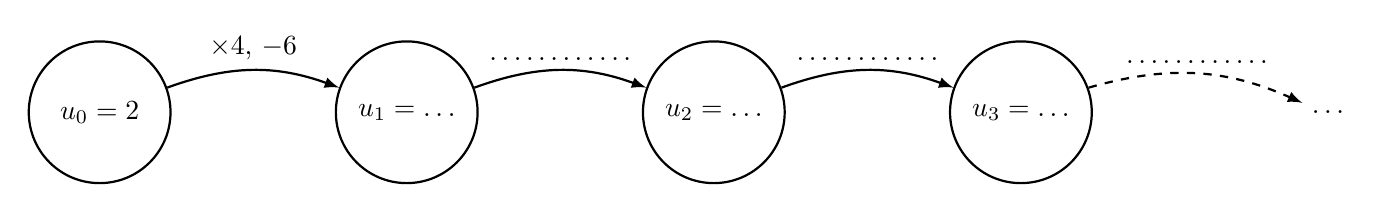
\begin{tikzpicture}[scale=1.3]
\node[draw,circle,thick, minimum size=18mm] (W0) at (-3,0) {$u_0=2$};
\node[draw,circle,thick, minimum size=18mm] (W1) at (0,0) {$u_1=\ldots$};
\node[draw,circle,thick, minimum size=18mm] (W2) at (3,0) {$u_2=\ldots$};
\node[draw,circle,thick, minimum size=18mm] (W3) at (6,0) {$u_3=\ldots$};
\node (W4) at (9,0) {$\ldots$};
\draw[->,>=latex,thick] (W0) to[bend left=20] node[midway,above]{$\times 4$, $-6$} (W1);
\draw[->,>=latex,thick] (W1) to[bend left=20] node[midway,above]{$\makebox[2cm]{\dotfill}$} (W2);
\draw[->,>=latex,thick] (W2) to[bend left=20] node[midway,above]{$\makebox[2cm]{\dotfill}$} (W3);
\draw[->,>=latex,thick,dashed] (W3) to[bend left=20] node[midway,above]{$\makebox[2cm]{\dotfill}$} (W4);
\end{tikzpicture}

\item Compléter alors la relation de récurrence suivante: $\left\{ \begin{matrix} u_0=\ldots \\ u_{n+1}= \ldots u_n \ldots \end{matrix} \right.$

\item Soit $w$ une suite telle que $w_0=3$ et pour $n \in \N$, $w_{n+1}=(w_n)^2-n$. Calculer:
\begin{itemize}
\item $w_1=$ \dotfill
\item $w_2=$ \dotfill
\item $w_3=$ \dotfill
\item $w_4=$ \dotfill
\end{itemize}
\item Vrai ou faux? La suite $w$ est décroissante. \makebox[3cm]{\dotfill}
\end{enumerate}

\end{exercice}

\begin{exercice} \
\begin{enumerate}
\item Déterminer l'équation réduite de la droite passant par $A(-2;1)$ et $B(1;7)$.

\points 3

\item Soit $f:x \mapsto 7x+21$. Montrer que le point $C(-3;0)$ appartient à la droite associée à $f$.

\points 2

\end{enumerate}
\compo[0.5]
{
\begin{enumerate}[start=3]
\item Dresser le tableau de signes de $f$:

\points 1

\end{enumerate}
}
{
\begin{centrer}
\begin{tikzpicture}
\tkzTabInit[lgt=1.5,espcl=1.5]{/1,/1}{,,,}
\end{tikzpicture}
\end{centrer}
}
\end{exercice}

\begin{exercice} \

\compo[0.7]
{
On se donne la parabole $\mathscr P$ ci-contre, et $f:x \mapsto ax^2+c$ la fonction de degré deux associée.
\begin{enumerate}
\item Quel est le signe de $a$? \dotfill
\item Donner la valeur de $c$: \dotfill
\item Placer le sommet de $\mathscr P$ et préciser ses coordonnées: \dotfill
\item Quel est l'axe de symétrie de $\mathcal P$? \dotfill
\item Donner les deux racines de $f$: \dotfill
\item En utilisant le point $A(2;4)$, déterminer $a$, et en déduire l'équation de $\mathscr P$, sous forme développée puis factorisée.
\end{enumerate}
}
{
\begin{centrer}
\begin{tikzpicture}
\begin{axis}[
styleglobal,
width=0.9*\linewidth,
xmin=-4, xmax=4,
ymin=-5, ymax=5,
xtick distance=1,
ytick distance=1,
]
\addplot[styleplot,domain=(-4:4)]{(2*x^2-4} node[pos=0.6,below right]{$\mathscr P$};;
\end{axis}
\end{tikzpicture}
\end{centrer}
}
\points 5
\end{exercice}

\begin{exercice} \

\compoligne
{
\begin{enumerate}
\item Tracer les droites $d_1$ et $d_2$ d'équations:
$$d_1:y=-2x+3 \ \text{ et } \ d_2:y=\frac 2 3 x+1$$
\end{enumerate}
\begin{centrer}
\begin{tikzpicture}
\begin{axis}[
styleglobal,
width=0.8*\linewidth,
xmin=-2, xmax=4,
ymin=-2, ymax=4,
xtick distance=1,
ytick distance=1,
%major grid style={line width=1pt},
]
\end{axis}
\end{tikzpicture}
\end{centrer}
}
{
\begin{enumerate}[start=2]
\item Déterminer l'équation des droites $d_3$ et $d_4$.
$$\vphantom{\frac 2 3}d_3:y=\hspace{2cm} \text{ et } d_4:y=\hspace{2cm}$$ %vphantom pour l'espacement
\end{enumerate}
\begin{centrer}
\begin{tikzpicture}
\begin{axis}[
styleglobal,
width=0.8*\linewidth,
xmin=-2, xmax=4,
ymin=-2, ymax=4,
xtick distance=1,
ytick distance=1,
%major grid style={line width=1pt},
]
\addplot[styleplot]{3*x-0.5} node[pos=0.55,right] {$d_3$};
\addplot[color=blue,styleplot,densely dotted]{-0.5*x+1} node[pos=0.8,below left] {$d_4$};
\end{axis}
\end{tikzpicture}
\end{centrer}
}
\end{exercice}

\begin{exercice} \

\compo[0.4]
{
\begin{center}
\strut Questions 2 et 3
\begin{tikzpicture}
\begin{axis}[
styleglobal,
width=0.9*\linewidth,
xmin=-2.5, xmax= 6.5,
ymin=-1.5, ymax=4.5,
xtick distance=1,
ytick distance=1,
]
\addplot[styleplot,tension=0.7] plot coordinates {(-2,4) (0,-1) (1,0.5) (2,-1) (4,2) (6,3)} node[pos=0.9,above left] {$\mathscr C_f$}  \pointsextremites;
\end{axis}
\end{tikzpicture}

\vspace{3mm}
Questions 4 et 5
\begin{tikzpicture}
\begin{axis}[
styleglobal,
width=0.9*\linewidth,
xmin=-2.5, xmax= 6.5,
ymin=-1.5, ymax=4.5,
xtick distance=1,
ytick distance=1,
]
\addplot[styleplot,tension=0.7] plot coordinates {(-2,4) (0,-1) (1,0.5) (2,-1) (4,2) (6,3)} node[pos=0.9,above left] {$\mathscr C_f$}  \pointsextremites;
\end{axis}
\end{tikzpicture}
\end{center}
}
{
On a représenté une fonction $f$ sur le repère ci-contre. Des constructions sont demandées pour les questions indiquées.
\begin{enumerate}
\item L'ensemble de définition de $f$ est $\dotfill$
\item L'image de 2 est \dotfill
\item L'image de -1 est \dotfill
\item $1$ a pour antécédent(s) \dotfill
\item $2,5$ possède \makebox[3cm]{\dotfill} antécédent(s).
\item Dresser un tableau de signes de la fonction $f$.
\end{enumerate}
\begin{center}
\begin{tabularx}{0.9\linewidth}{|c|X|} \hline
\rule{0pt}{25pt} & \\ \hline
\phantom{f(x)} & \rule{0pt}{25pt}\\ \hline
\end{tabularx}
\end{center}
}
\end{exercice}

\newpage
\begin{exercice}
Soit $f:[0;5] \rightarrow \R$ la fonction qui à $x$ associe $\frac {10x-2}{x+2}$.

\compo[0.7]
{
\begin{enumerate}
\item Compléter le tableau de valeurs suivant, en arrondissant au dixième près:

\begin{center}
\begin{tabularx}{0.95\linewidth}{|c|*{6}{Y|}} \hline
$x$ & $0$ & $1$ & $2$ & $3$ & $4$ & $5$ \\ \hline
$f(x)$ & & & & & & \rule{0pt}{8mm} \\ \hline
\end{tabularx}
\end{center}
\item Tracer sur le repère ci-contre la représentation graphique de $f$.
\end{enumerate}
}
{
\vspace{-1.5cm}
\begin{tikzpicture}
\begin{axis}[
styleglobal,
width=\linewidth,
xmin=-0.5, xmax= 5.5,
ymin=-1.5, ymax=7.5,
xtick distance=1,
ytick distance=1,
]

\end{axis}
\end{tikzpicture}
}
\end{exercice}

\begin{exercice}
Voici trois situations et trois calculs. Associer chaque situation à un calcul en imaginant une question.
\begin{enumerate}
\item Un ordinateur coute $450$\euro{}. Un commerçant accorde une remise de $6\%$.
\item La longueur d'une piste d'ULM est $450$m. On l'augmente de $6 \%$.
\item $6 \%$ des 450 pompiers d'une ville ont moins de 20 ans.
\end{enumerate}

\noindent \hfill A. $450 \times 1,06$ \hfill B. $450 \times 0,06$ \hfill C. $450 \times 0,94$ \hfill \

\points 6
\end{exercice}

\begin{exercice}
En janvier 2019, une entreprise renouvelle son parc de tablettes tactiles. La tablette choisie affiche une autonomie de 8 heures. Une étude montre que l'autonomie de la batterie baisse de 15\% chaque année d'utilisation.

Soit $n$ un entier naturel. On modélise le nombre d'heures d'autonomie de cette tablette pour l'année $2019+n$ par une suite $(a_n)$. Ainsi $a_0=8$. \textit{On arrondira les résultats au centième d'heure.}

\begin{enumerate}
\item Déterminer l'autonomie de la batterie en 2020 puis en 2021.

\points 2

\item Compléter: $a_{n+1}=a_n \times \ldots$
\item Déterminer l'autonomie de la batterie en 2023, puis en 2030. \textit{On utilisera la calculatrice.}

\points 3
\end{enumerate}
\end{exercice}

\end{document}
